\providecommand{\main}{../main}
\documentclass[\main/main.tex]{subfiles}
\graphicspath{{../images/}}
% \addbibresource{../ref/ref.bib}
\begin{document}
\section{
    場の理論における対称性
}
古典論におけるNoetherの定理は運動方程式のもとで成り立つ。
一方量子論
\footnote{
    ここでの量子論とは経路積分をするという意味である。
    統計的場の理論もこの意味では量子的である。
}
では運動方程式を満たさない場の配位を考慮に入れる必要がある。
この章では場の理論におけるNoetherの定理の対応物であるWard-Takahashi恒等式を導き、共形不変性によって相関関数がどのように制限されるかを見る。
\subsection{
    Schwinger-Dyson方程式
}
まず運動方程式$\δ*{S}{ϕ}=0$が量子論においてどのように補正を受けるのかを見る。
場の微小変換
\begin{align}
    ϕ'(x) = ϕ(x) + δϕ(x)
\end{align}
を考える。
$δϕ(x)$は$ϕ(x)$に依存しない場とする。
ここで経路積分に関する恒等式
\begin{align}
    ∫\𝒟{ϕ'} F[ϕ']\e^{-S[ϕ']}
    = ∫\𝒟{ϕ} F[ϕ]\e^{-S[ϕ]}
    \label{path integral identity}
\end{align}
に注目する。これは単純な積分変数の取り替えなので、常に成り立つ。
左辺から右辺を引く。
$δϕ(x)$が$ϕ(x)$に依存しないことから$\d{ϕ'(x)}=\d{ϕ(x)}$であり、これを掛け合わせて$\𝒟{ϕ'} = \𝒟ϕ$が成り立つので、
\begin{align}
   ∫\𝒟ϕ∫\d^d{x}\Q(
        \δ{F[ϕ]}{ϕ(x)}δϕ(x)
        -\δ{S[ϕ]}{ϕ(x)}F[ϕ]δϕ(x)
   )\e^{-S[ϕ]}
   = 0
\end{align}
となる。
ただし、積分領域の境界で$δϕ(x)=0$として、表面項を無視した。
両辺を分配関数で割ると、
\begin{align}
    \⟨\δ{S[ϕ]}{ϕ(x)}F[ϕ]\⟩=\⟨\δ{F[ϕ]}{δϕ}\⟩
\end{align}
となる。
特別な場合として、$F[ϕ] = ϕ(x₁)⋯ϕ(xₙ)$とした以下の式はSchwinger-Dyson方程式と呼ばれる。
\begin{align}
    \⟨\δ{S[ϕ]}{ϕ(x)}ϕ(x₁)⋯ϕ(xₙ)\⟩
    = ∑_{j=1}^n δ(x-xⱼ)\⟨ϕ(x₁)⋯\cancel{ϕ(xⱼ)}⋯ϕ(xₙ)\⟩
    \label{Schwinger-Dyson equation}
\end{align}
つまり運動方程式$\δ*{S}{ϕ(x)}$は古典的にはゼロだが、量子論ではゼロではなく、演算子$ϕ(x')$と同一点にあるときにデルタ関数$δ(x-x')$に比例する寄与をもつ。
これを接触項と呼ぶ。

ここでNoetherの定理$∂_μJ^μ=0$が古典的な等式、すなわち運動方程式のもとでの等式であったことを思い出すと、量子論では接触項によって補正されることが分かる。
\subsection{
    Ward-Takahashi恒等式
}
微小な座標変換
\begin{align}
    {x'}^μ - x^μ = ε^μ(x) = ε^a(x)X_ax^μ
\end{align}
とそれに伴う内部空間の微小変換
\begin{align}
    𝝓'(x') - 𝝓(x) = G𝝓(x) = ε^a(x)G_a𝝓(x),
\end{align}
を考える。
ここで、$X_a=X_a^μ∂_μ$は微分演算子であり、$G_a$はLie群の生成子である。
また
\begin{align}
    𝝓'(x) - 𝝓(x) ≕ ε^a δ𝝓_a(x)
    = ε^a(x)(X_a+G_a)𝝓(x)
\end{align}
と書くことにする。
グローバル変換$ε^a(x) = ε^a$に対して作用が不変であるとき、相関関数に課される制限を求める。

出発点は先ほどと同様で恒等式
\begin{align}
    ∫\𝒟{𝝓'} F[𝝓']\e^{-S[𝝓']}
    = ∫\𝒟{𝝓} F[𝝓]\e^{-S[𝝓]}
    % \label{path integral identity}
\end{align}
である。
左辺は
\begin{align}
    &
    ∫\𝒟{𝝓'} F[𝝓']\e^{-S[𝝓']}
    \∅ &
    = ∫\𝒟{𝝓'}\Q(
        F[𝝓]
        + ∫\d^d{x}ε^a(x)\δ{F[𝝓]}{𝝓(x)}⋅δ𝝓_a(x)
        - F[𝝓]δS[𝝓]
    )\e^{-S[𝝓]}
\end{align}
と変形できる。
ここで、作用の変化はNoetherカレント$J_a^μ$によって
\begin{align}
    δS = ∫\d^d{x}J_a^μ(x)∂_με^a(x)
    = -∫\d^d{x}ε^a(x)∂_μJ_a^μ(x)
    \label{CWTI: δS}
\end{align}
と書ける。ただし、積分領域の境界で$ε^a(x)=0$とし、表面項を無視した。

ここで、経路積分測度について$\𝒟{𝝓'}=\𝒟𝝓$が成り立つとする。
この仮定の妥当性については後で改めて考える。
すると、(\ref{path integral identity})は
\begin{align}
    ∫\d^d{x}ε^a(x)∫\𝒟𝝓 \Q(\δ{F[𝝓]}{𝝓(x)}⋅δ𝝓_a(x) + F[𝝓]∂_μ J_a^μ(x) )\e^{-S[𝝓]} = 0
\end{align}
と書ける。
$ε^a(x)$は任意なので、$∫\d^d{x}ε^a(x)$を除くことができる。さらに両辺を分配関数で割ると、
\begin{align}
    \⟨∂_μJ_a^μ(x)F[𝝓]\⟩
    = -\⟨\δ{F[𝝓]}{𝝓(x)}⋅δ𝝓_a(x)\⟩
    \label{CWTI: generalized WTI}
\end{align}
となる。
ここで、$F[𝝓] = 𝒪₁(x₁)⋯𝒪_N(x_N)$とすることで、対称性によって相関関数に課される条件が得られる。
ただし、$𝒪ₙ(xₙ)$は$𝝓(xₙ),∂_μ𝝓(xₙ),…$の関数として表される局所場である。
\footnote{
    同一点の場の積をとると一般に相関関数が発散してしまうので、複合場は無限大の定数を差し引いて定義される。
}
また
\begin{align}
    \δ{𝒪ₙ(xₙ)}{𝝓(x)}⋅δ𝝓_a(x)
    &
    ≕ δ(x-xₙ)𝒬_a𝒪ₙ(x)
\end{align}
と定義すると
\begin{align}\tcboxmath{
    \⟨∂_μJ_a^μ(x)𝒪₁(x₁)⋯𝒪_N(x_N)\⟩
    = -∑_{n=1}^N δ(x-xₙ)\⟨
        𝒪₁(x₁)⋯𝒬_a𝒪ₙ(x)⋯𝒪_N(x_N)
    \⟩
    \label{CWTI: WTI}
}\end{align}
が得られる。この式をWard-Takahashi恒等式と呼ぶ。

次に、保留しておいた経路積分測度の変換について考える。
例えば$δ𝝓_a(x)=G_a𝝓(x)$のとき、素朴には
\begin{align}
    \𝒟{𝝓'} =\𝒟𝝓 ∏_x\det(1+ε^aG_a)^{ρ\d^dx}
    ≈\𝒟𝝓\exp∫\d^dxρε^a\tr G_a
\end{align}
と書ける。
ここで$ρ$は自由度の密度であり、格子正則化の場合は格子間隔$a$によって$ρ=1/a^d$と書ける。
もし右辺の指数関数の中身が$0$になるならば、経路積分測度は不変である。
このためには$\tr G_a= 0$が成り立てば良いが、場の理論では$ρ → ∞$とするために$∞⋅0$となって不定になってしまう。
したがって、極限を真面目に議論する必要がある。
もしその結果$\𝒟{𝝓'}≠\𝒟𝝓$となったならば、量子異常(アノマリー、対称性の量子的破れ)が存在すると言う。
\footnote{
    経路積分のJacobianから量子異常を導く方法はFujikawaの方法と呼ばれる。
    詳しくは\cite{Fujikawa_2001}などを参照してほしい。
}
このとき
\begin{align}
    \⟨∂_μJ_a^μ\⟩ ≠ 0
\end{align}
となる。つまり古典的には保存するカレントが量子的には保存しなくなる。
平坦な時空の共形変換を考える上では量子異常は考えなくてよいので、
\footnote{
    並進対称性や回転対称性はこれらを保つ正則化が構成できるので、極限の過程で常に経路積分測度を不変にできる。
    スケール変換の場合、経路積分測度を不変にするためには単純な座標変換ではなく、くりこみ変換を考える必要がある。
    このとき一般に異常次元が発生して古典的な次元に対するスケール不変性が破れるため、この意味でスケール不変性に量子異常があると言うことがある。
    ただし、その場合も固定点では量子的なスケール不変性が成り立っている。
    特殊共形変換の場合は経路積分測度を不変にするために一般化されたくりこみ変換を考える。これは特殊共形変換と粗視化を組み合わせたものである。
    また、曲がった時空における共形対称性(正確にはWeyl対称性)は量子的に破れること(Weylアノマリー)があるが、平坦な時空では考える必要がないらしい。
}
これ以上深入りはしないことにする。
% \footnote{
%     並進変換は$\𝒟𝝓=∏_x𝝓(x)$のラベル$x$を変えるだけなので、測度を変えない。また回転変換は内部空間の回転を伴うが、行列式が1なのでこれも測度を変えない。
%     スケール変換や特殊共形変換の場合は単なる座標変換ではなく粗視化を伴うくりこみ変換を考えることで、$\𝒟{𝝓'}=\𝒟𝝓$が成り立つ。
% }
% これに伴って作用は
% \begin{align}
%     δS = δS_\rm{classical} + δS_\rm{quantum}
% \end{align}
% のように変化する。
% ここからスケール変換に対し$δS_\rm{classical} = 0$を課して得られる場の正準次元と、$δS = 0$によって得られる場の次元が異なる可能性がある。
% 正準次元解析を破るような$δS_\rm{quantum}$による次元を異常次元と呼ぶ。

\subsection{
    トポロジカル演算子
}
% Ward-Takahashi恒等式を演算子形式に直してみる。
% まず、Noetherチャージを、
% \begin{align}
%     \^Q_a(t) = ∫\d^{d-1}{𝒙}\^J_a^0(t,𝒙)
% \end{align}
% によって定義する。
% ここで$\^J_a^0(t,𝒙)$はHeisenberg表示の演算子である。
% (\ref{CWTI: WTI})において$N=0$として、$t'$から$t$まで積分すると、
% \begin{align}
%     \⟨Q_a(t)-Q_a(t')\⟩
%     = ⟨φ_f|\^U(t_f,0)\Q(\^Q_a(t)-\^Q_a(t'))\^U(0,t_i)|φ_i⟩
%     = 0
% \end{align}
% が成り立つ。
% 境界条件$φ_f,φ_i$は任意に取れるので、演算子の等式として$\^Q_a(t)=\^Q_a(t')$が成り立つ。
% つまりNoetherチャージは時間に依存せず、これを$\^Q_a$と書くことができる。
% 次に、(\ref{CWTI: WTI})を$tₙ-δt$から$tₙ+δt$まで積分すると、
% \begin{align}
%     ∫^{tₙ+δt}_{tₙ-δt}\d^d{x}\⟨∂_μJ_a^μ(x)⋯𝒪ₙ(xₙ)⋯\⟩
%     &
%     =⟨0|𝖳^*⋯[\^Q_a,\^𝒪ₙ(xₙ)]⋯|0⟩
%     \∅ &
%     = -\⟨⋯𝒬_a𝒪ₙ(xₙ)⋯\⟩
% \end{align}
% となる。ここで、$t_n-δt$から$t_n+δt$の間に他の演算子が挿入されていないとした。
% ここから、演算子の等式として、
% \begin{align}\tcboxmath{
%     [\^Q_a,\^𝒪(x)] = -𝒬_a\^𝒪(x)
%     \label{CWTI: Noether charge as generator}
% }\end{align}
% が成り立つ。わかりにくい表記を用いているが、$\^Q_a$はHilbert空間に作用する演算子であり、$𝒬_a$は局所場の完全系が張る空間に作用する微分演算子である。

% 以上は時間一定面での議論だった。さらにNoetherチャージを一般の超曲面に拡張しよう。
時空上の領域$B$に対し、その境界$∂B$の上でのNoetherチャージを
\begin{align}
    Q_a(∂B)
    ≔ -∫_{∂B}\d{S_μ} J_a^μ(x)
    = -∫_B \d^d{x} ∂_μJ_a^μ(x)
\end{align}
と定義する。
Ward-Takahashi恒等式から$B$の内部に演算子が含まれていない場合、$Q_a(∂B)$の期待値は$0$である。
\begin{align}
    \⟨Q_a(∂B)∏_{n: xₙ ∉ B}𝒪ₙ(xₙ)\⟩ = 
    \graph[scale=0.3]{CWTI-Q.pdf} = 0.
    \label{CWTI: ⟨Q(∂B)⟩=0}
\end{align}
これを複素関数論におけるCauchyの積分定理のように使って、$∂B$を連続的に自由に変形することができる。
ここから$Q_a(∂Bₙ)$をトポロジカル演算子と呼ぶ。
% \footnote{
%     (余談)
%     場の量子論において、対称性は余次元$1$のトポロジカル演算子に対応する。
%     この考えを拡張して余次元が$2$以上のトポロジカル演算子が存在するときに、高次対称性が成り立つと言う。
%     高次対称性については日高義将さんの講義ノート(\url{https://ribf.riken.jp/~hidaka/files/lecture/summer2019.pdf})が参考になる。
% }
例えば、以下のような変形が可能である。
\begin{figure}[H]
    \centering
    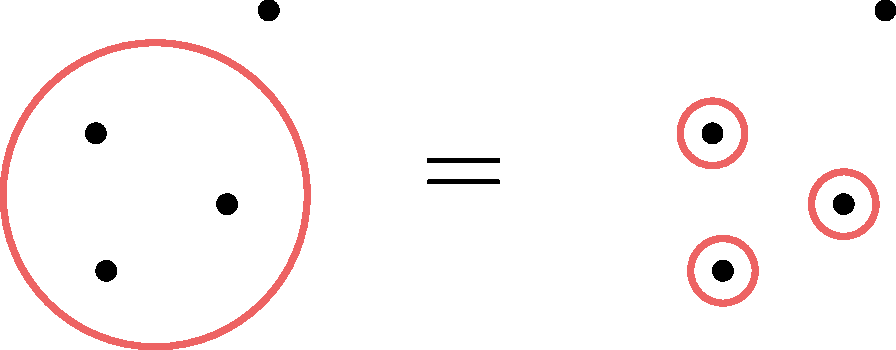
\includegraphics[width=0.3\hsize]{../images/topological transformation.pdf}
    \caption{トポロジカル演算子の変形}
\end{figure}
$B$を$x$まわりの微小な閉曲面とすると、Ward-Takahashi恒等式を$B$の内部で積分することで、
\begin{align}
    Q_a(∂B)𝒪(x) = 𝒬_a𝒪(x)
\end{align}
% \begin{align}
%     \graph[scale=0.3]{CWTI-QO(x)}
% \end{align}
を得る。ただし、これは任意の境界条件で期待値を取った時に成り立つという意味である。
以降は$∂B$を省略して$Q_a𝒪(x)$と書いたとき、$Q_a$は$x$まわりの微小な閉曲面でのトポロジカル演算子を表すとする。

同じことを通常の量子化
\footnote{
    時間一定面のHilbert空間に対する演算子形式のことを言っている。
    後で説明する動径量子化と対比するならば時間量子化だが、これもまた紛らわしい言い方だろう。
}
の枠組みでも見ておく。
Ward-Takahashi恒等式を領域$t+δt ≥ t' ≥ t-δt$上で積分する。この領域の内部に一つの局所演算子$𝒪(x)$のみがあったとすると、
\begin{align}
    Q_a(∂B) 𝒪(x) = Q_a(t+δt)𝒪(x) - Q_a(t-δt)𝒪(x) = -𝒬_a𝒪(x)
\end{align}
と書ける。ここで、
\begin{align}
    Q_a(t) = -∫\d^{d-1}{𝒙}J_a^0(t,𝒙)
\end{align}
と定義した。
これを時間順序に直すことで演算子の等式
\begin{align}
    \^Q_a(t+δt)\^𝒪(x) - \^𝒪(x)\^Q_a(t-δt) = 𝒬_a\^𝒪(x)
\end{align}
を得る。
ここで$\^𝒪(x) = 1$とおくと、$\^Q_a(t)$が$t$によらないことが分かるから、
\begin{align}
    \^Q_a(∂B)\^𝒪(x) = [\^Q_a,\^𝒪(x)] = 𝒬_a\^𝒪(x)
    \label{CWTI: operator ward identity}
\end{align}
と書ける。
トポロジカル演算子は交換関係$[\^Q_a,\^𝒪(x)]$の量子化の方法によらない定義を与えていると言える。
\begin{figure}[H]
    \centering
    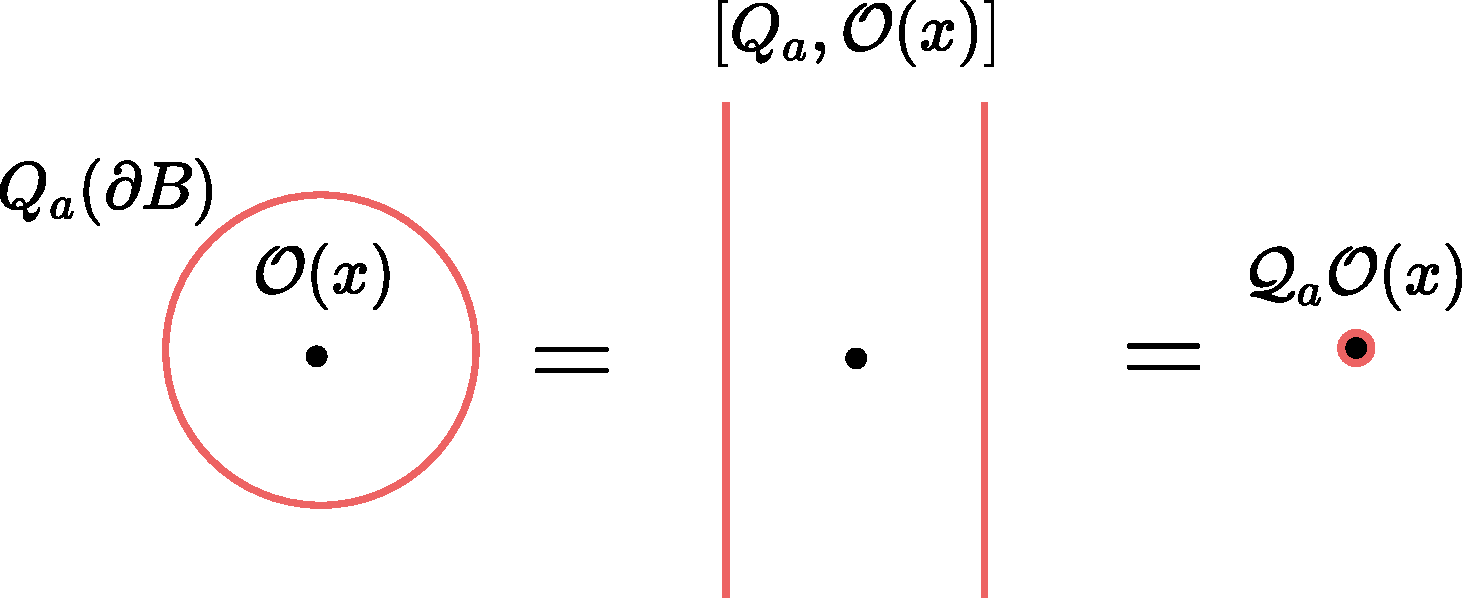
\includegraphics[width=0.5\hsize]{CWTI-QO(x).pdf}
    \caption{交換関係のトポロジカルな定義}
\end{figure}
$\^Q_a$をHamiltonianとすれば、(\ref{CWTI: operator ward identity})はEuclid空間におけるHeisenbergの運動方程式
\begin{align}
    [\^H,\^𝒪(t,𝒙)] = \∂{t}\^𝒪(t,𝒙)
\end{align}
となる。
またこれを積分することで、
\begin{align}
    \^𝒪(t,𝒙) = \e^{\^H t}\^𝒪(0,𝒙)\e^{-\^H t}
\end{align}
が得られる。

\subsection{
    積の順序についての注意
}
2回の微小な変換の$x → x + ε^aX_a → x + ε^aX_a + {ε'}^bX_b$に対して
Ward-Takahashi恒等式の議論を繰り返すと
\begin{align}
    Q_aQ_b𝒪(x) = 𝒬_b 𝒬_a 𝒪(x)
\end{align}
となる。ここで、トポロジカル演算子の積をとるときは左が外側で右が内側にあると約束する。
ここで、$𝒬_a,𝒬_b$微分演算子であり、変換の合成の順序と積の順序が逆であることに注意する。
したがってトポロジカル演算子と微分演算子の順序は逆であり、交換関係は符号が反転する。
\begin{align}
    [Q_a,Q_b]𝒪(x) = -[𝒬_a,𝒬_b]𝒪(x)
\end{align}
共形変換の生成子について、後で用いる交換関係を改めて書いておく。
\begin{align*} 
    &
    [D,P_μ] = P_μ,\␣
    [D,K_μ] = -K_μ,
    \\ &
    [K_μ,P_ν] = 2δ_{μν}D-2M_{μν}
    \\ &
    [P_μ,M_{νρ}] = δ_{μν}P_ρ - δ_{μρ}P_ν
\end{align*}

\subsection{
    共形変換に対するWard-Takahashi恒等式
}
\subsubsection*{
    並進
}
以下では、具体的に共形変換に対応するNoetherチャージを構成しよう。
並進対称性の場合、Ward-Takahashi恒等式は、
\begin{align}\tcboxmath{
    \⟨∂_μ{T^μ}_ν(x)𝒪₁⋯𝒪_N\⟩
    = -∑_{n=1}^N δ(x-xₙ)\⟨𝒪₁⋯∂_ν𝒪ₙ⋯𝒪_N\⟩
    \label{CWTI: translation WTI}
}\end{align}
となる。
Noetherチャージは4元運動量であり、
\begin{align}
    P_μ = -∫\d{S_ν}{T^ν}_μ
\end{align}
と定義される。Ward-Takahashi恒等式から
\begin{align}
    P_μ𝒪(x) = ∂_μ 𝒪(x)
\end{align}
が成り立つ。また
\begin{align}\tcboxmath{
    𝒪(x) = \e^{x⋅P}𝒪(0)
}\end{align}
と書ける。
同じことを演算子形式で書くと、
\begin{align}
    \^𝒪(x) = \e^{[x⋅\^P,]}\^𝒪(0) = \e^{x⋅\^P}\^𝒪(0)\e^{-x⋅\^P}
\end{align}
となる。
\subsubsection*{
    回転
}
次に回転変換$x^μ → x^μ - b^{μν}x_ν,b^{νμ}=-b^{μν}$に対し、
Ward-Takahashi恒等式は
\begin{align}
    &
    \⟨∂_ρ(x^νT^{ρμ}-x^μT^{ρν})𝒪₁⋯𝒪_N\⟩
    \∅ &
    = -∑_{n=1}^N 
        δ(x-xₙ)\⟨𝒪₁⋯(x^ν∂^μ-x^μ∂^ν+𝒮^{μν})𝒪ₙ⋯𝒪_N\⟩
    \label{rotation WTI}
\end{align}
となる。
$𝒮^{μν}$は$𝔰𝔬(d)$の表現で、$𝒪ₙ(x)$がスピンをもつ多成分の場の場合に必要である。
トポロジカルな演算子は
\begin{align}
    M^{μν}
    ≔ -∫\d{S_ρ}(x^νT^{ρμ}-x^μT^{ρν})
\end{align}
と定義される。ここで$T^{ρμ}$は対称に改良されたエネルギー運動量テンソルとする。
(\ref{rotation WTI})を積分することで、
\begin{align}
    M^{μν}𝒪(x) = (x^ν∂^μ - x^μ∂^ν + 𝒮^{μν})𝒪(x)
\end{align}
が成り立つ。また(\ref{CWTI: translation WTI})から
\begin{align}\tcboxmath{
    \⟨(T^{νμ}-T^{μν})𝒪₁⋯𝒪_N\⟩
    = -∑_{n=1}^N δ(x-xₙ)\⟨𝒪₁⋯𝒮^{μν}𝒪ₙ⋯𝒪_N\⟩
}\end{align}
と書ける。
つまり、$T^{νμ}-T^{μν}$は古典的にはゼロだが、量子的には接触項による補正が加わる。
\subsubsection*{
    スケール変換
}
次にスケール変換$x^μ → (1-λ)x^μ$に対し、Ward-Takahashi恒等式は
\begin{align}
    &
    \⟨∂_μ(x_νT^{μν}(x))𝒪₁⋯𝒪_N\⟩
    \∅ &
    = -∑_{n=1}^N δ(x-xₙ)\⟨𝒪₁⋯(x⋅∂+Δₙ)𝒪ₙ⋯𝒪_N\⟩
    \label{scale WTI}
\end{align}
となる。
$Δₙ$は一般に行列になり得るが、実数固有値によって対角化可能であることを仮定する。
ここではすでに対角化されているとして$Δₙ$を実数とおく。
トポロジカルな演算子は
\begin{align}
    D = -∫\d{S_μ}x^νT^{μν}
\end{align}
と定義される。ここで$T^{μν}$はトレースレスに改良されたエネルギー運動量テンソルとする。
(\ref{scale WTI})を積分すると、
\begin{align}
    D𝒪(x) = (x⋅∂+Δ)𝒪(x)
\end{align}
が成り立つ。
また(\ref{CWTI: translation WTI})から
\begin{align}\tcboxmath{
    \⟨T^μ_μ(x)𝒪₁(x₁)⋯𝒪_N(x_N)\⟩
    = -∑_{n=1}^N Δₙδ(x-xₙ)\⟨𝒪₁(x₁)⋯𝒪_N(x_N)\⟩
}\end{align}
である。
つまり、$T^μ_μ$は古典的にはゼロだが、量子的には接触項による補正が加わる。

% \subsection{
%     エネルギー運動量テンソルの交換関係
% }
% \begin{align}
%     T^{μν}T^{ρσ}
%     = \f{x^μ}{S_{d-1}|x|^d} ∂^νT^{ρσ} + ⋯
% \end{align}
% \begin{align}
%     T^μ_μT^{ρσ}
%     = \f{x⋅∂+Δ}{S_{d-1}|x|^d}T^{ρσ}+
% \end{align}

% \printbibliography
\end{document}